\subsection{Descrição de \textit{software}}\label{subsec:software}

O \textit{software} do sistema é dividido em dois níveis de processamento:
o \textit{firmware} embarcado no STM32G070, responsável pelo controle em
tempo real dos atuadores e sensores, e o programa de alto nível executado
no Raspberry Pi~3B, responsável pela supervisão do sistema, leitura de
código QR e comunicação com o microcontrolador.

% ==================================================================
\subsubsection{\textit{Firmware} do STM32G070}
% ==================================================================

O \textit{firmware} foi desenvolvido em linguagem C utilizando os
\textit{drivers} HAL da STMicroelectronics no ambiente STM32CubeIDE. Sua
estrutura principal é composta por uma rotina de inicialização, um laço
principal (\textit{loop} infinito) e uma Máquina de Estados Finitos (FSM).

\paragraph{Rotina de inicialização.}
Antes de entrar no laço principal, o \textit{firmware} executa uma rotina
de bloqueio que aguarda simultaneamente duas condições: (i) todos os quatro
sensores laser devem operar na frequência esperada de 200\,Hz, e (ii) o
Raspberry Pi deve enviar o byte de \textit{handshake} \texttt{SYS\_RDY}
(\texttt{0x10}). Durante esse período, um LED de depuração indica o estado
do sistema: pisca a 100\,ms se os sensores ainda não estiverem prontos, e a
500\,ms quando aguarda apenas o \textit{handshake}. Ao receber o sinal do
Raspberry Pi, o STM32G070 responde com \texttt{SYS\_INIT} (\texttt{0x01})
e ingressa no laço principal.

\paragraph{Leitura dos sensores laser.}
A leitura dos sensores é baseada em detecção síncrona por ausência de
portadora. O TIM15 gera um PWM de 200\,Hz para modular os quatro lasers
simultaneamente. O TIM3, em modo \textit{Input Capture} com DMA, mede a
frequência do sinal retornado por cada LDR. Se a frequência capturada
corresponde à portadora (200\,Hz), o feixe está livre; se a captura retorna
zero (ausência de sinal), há um objeto interrompendo o feixe. O laço
principal chama \texttt{getSensorsReadings()} a cada intervalo definido,
atualizando as variáveis de estado \texttt{SENSn\_freq} e
\texttt{SENSn\_flag} para cada sensor $n \in \{1,2,3,4\}$.

\paragraph{Controle do motor de passo.}
O motor de passo NEMA 22 é acionado via TIM6, que opera a 1\,MHz e gera
interrupções periódicas para o controle preciso dos pulsos enviados ao pino
STEP do \textit{driver} A4988. O sentido de rotação é determinado pelo pino
DIR, e o pino SLEEP controla o engajamento do eixo. Funções auxiliares como
\texttt{stepperMove()}, \texttt{stepperSetSpeed()},
\texttt{stepperStopEngaged()} e \texttt{stepperStopDisengaged()} encapsulam
o controle do motor, permitindo que a FSM abstraia os detalhes de
temporização.

\paragraph{Controle do servo motor.}
O servo ES08MA é controlado pelo TIM16, que gera um PWM de 50\,Hz com
\textit{duty cycle} variável. A função \texttt{SetServoAngle(angle)} mapeia
o ângulo desejado (em graus) para o valor de comparação do registrador do
\textit{timer}, com largura de pulso variando de 600\,µs (0°) a 2300\,µs
(180°). No contexto da FSM, a cancela opera em dois estados: fechada (0°),
posicionando os objetos para a Rota~A, e aberta (45°), desviando-os para a
Rota~B.

\paragraph{Máquina de Estados Finitos (FSM).}
O fluxo de operação do sistema é controlado por uma FSM implementada na
função \texttt{FSM()}, chamada ciclicamente no laço principal. O diagrama
de estados é apresentado na Fig.~\ref{fig:fsm_diagram}. Os estados são:

\begin{figure}[!htpb]
    \centering
    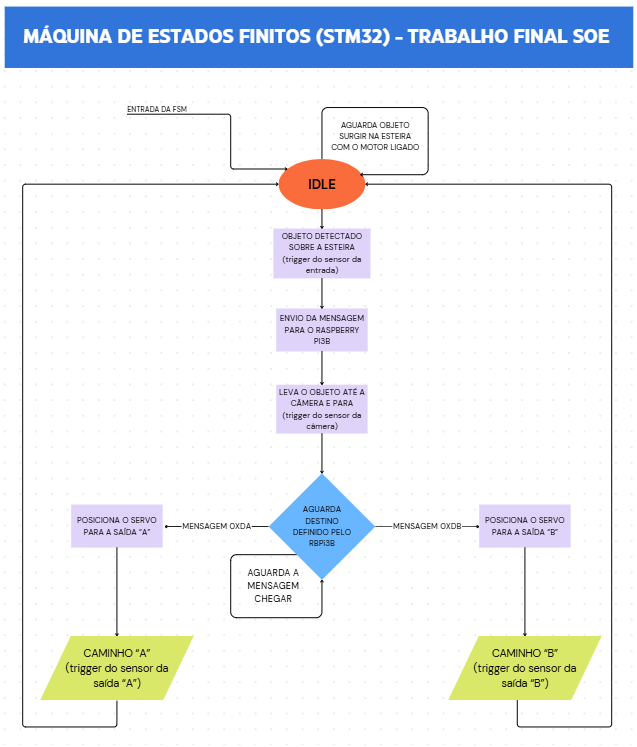
\includegraphics[width=0.35\textwidth]{figuras/fsm_flow.png}
    \caption{Diagrama de estados da FSM do \textit{firmware} do STM32G070.}
    \label{fig:fsm_diagram}
\end{figure}

\begin{itemize}
    \item \textbf{IDLE:} sistema aguardando objeto. Motor ligado, cancela
          fechada, \textit{flash} apagado;
    \item \textbf{OBJ\_DETECTED:} objeto detectado pelo sensor S1. Motor
          continua em movimento transportando o objeto até a zona de leitura;
    \item \textbf{CLASSIF\_REQUEST:} objeto parado sob o sensor S2 (zona de
          leitura). Motor para. \textit{Flash} aceso. STM32 envia
          \texttt{CLSS\_REQUEST} (\texttt{0xC0}) ao Raspberry Pi e aguarda
          resposta de roteamento;
    \item \textbf{ROUTE\_A:} Raspberry Pi enviou \texttt{ROUTE\_A}
          (\texttt{0xDA}). Cancela permanece fechada. Motor reinicia. STM32
          envia \texttt{ROUTE\_A\_FWRDNG} (\texttt{0xFA}) e aguarda detecção
          no sensor S3;
    \item \textbf{ROUTE\_B:} Raspberry Pi enviou \texttt{ROUTE\_B}
          (\texttt{0xDB}). Cancela abre (45°). Motor reinicia. STM32 envia
          \texttt{ROUTE\_B\_FWRDNG} (\texttt{0xFB}) e aguarda detecção no
          sensor S4;
    \item \textbf{DELIVERED:} sensor de saída detectou o objeto. Mensagem de
          entrega bem-sucedida enviada ao Raspberry Pi. Sistema retorna a
          IDLE.
\end{itemize}

\paragraph{Modo de depuração (\textit{DEBUG}).}
O \textit{firmware} implementa um modo de operação alternativo, ativado pelo
comando \texttt{DEBUG\_TOGGLE} (\texttt{0xDD}). Nesse modo, a FSM é suspensa
e o STM32G070 passa a responder exclusivamente a comandos assíncronos
enviados pelo Raspberry Pi, permitindo o acionamento individual de cada
atuador (\textit{flash}, cancela, motor de passo) para fins de diagnóstico e
validação. O STM32 também envia espontaneamente a telemetria dos quatro
sensores (\texttt{SENS\_STATUS}, \texttt{0x55}) sempre que o estado de algum
sensor muda.

\paragraph{Protocolo de comunicação UART.}
A comunicação entre o STM32G070 e o Raspberry Pi 3B segue um protocolo
proprietário desenvolvido para este projeto, operando a 115200\,bps
(8N1 — oito bits de dados, sem paridade, um \textit{stop bit}). O
recebimento é gerenciado por interrupção (\texttt{HAL\_UART\_Receive\_IT}),
garantindo que nenhum byte seja perdido durante a execução da FSM. A
estrutura dos quadros é definida conforme a Tabela~\ref{tab:uart_protocol},
e as principais mensagens do protocolo são apresentadas na
Tabela~\ref{tab:uart_messages}.

\begin{table}[!htpb]
\renewcommand{\arraystretch}{0.9}
\caption{Estrutura dos quadros UART.}
\label{tab:uart_protocol}
\centering
\footnotesize
\begin{tabular}{lp{4cm}}
\hline
\textbf{Direção} & \textbf{Formato} \\
\hline
RPi $\to$ STM32 (RX)      & \texttt{[0xAA][CMD]} ou \newline\texttt{[0xAA][0xE5][DATA]} \\
STM32 $\to$ RPi (TX ok)   & \texttt{[0x90][PAYLOAD]} \\
STM32 $\to$ RPi (TX erro) & \texttt{[0x91]} \\
\hline
\end{tabular}
\end{table}

\begin{table}[!htpb]
\renewcommand{\arraystretch}{0.8}
\caption{Mensagens do protocolo UART proprietário.}
\label{tab:uart_messages}
\centering
\footnotesize
\begin{tabular}{p{2.2cm}p{2.9cm}cc}
\hline
\textbf{Nome} & \textbf{Descrição} & \textbf{Valor} & \textbf{Dir.} \\
\hline
\multicolumn{4}{l}{\textit{Handshake}} \\
\texttt{SYS\_RDY}         & RPi sinaliza pronto          & \texttt{0x10} & RX \\
\texttt{SYS\_INIT}        & STM32 confirma               & \texttt{0x01} & TX \\
\hline
\multicolumn{4}{l}{\textit{Mensagens da FSM}} \\
\texttt{OBJ\_DETECTED}    & Objeto detectado (S1)        & \texttt{0xA0} & TX \\
\texttt{CLSS\_REQUEST}    & Solicita classificação       & \texttt{0xC0} & TX \\
\texttt{ROUTE\_A}         & Ordena rota A                & \texttt{0xDA} & RX \\
\texttt{ROUTE\_B}         & Ordena rota B                & \texttt{0xDB} & RX \\
\texttt{ROUTE\_A\_FWRDNG} & Confirm. encaminh. A         & \texttt{0xFA} & TX \\
\texttt{ROUTE\_B\_FWRDNG} & Confirm. encaminh. B         & \texttt{0xFB} & TX \\
\texttt{ROUTE\_A\_OK}     & Entrega concluída A          & \texttt{0xBA} & TX \\
\texttt{ROUTE\_B\_OK}     & Entrega concluída B          & \texttt{0xBB} & TX \\
\hline
\multicolumn{4}{l}{\textit{Controle assíncrono (modo DEBUG)}} \\
\texttt{LIGHT\_EN}        & Liga luminária               & \texttt{0xE1} & RX \\
\texttt{LIGHT\_DIS}       & Desliga luminária            & \texttt{0xD1} & RX \\
\texttt{GATE\_OPEN}       & Abre cancela (45°)           & \texttt{0xE2} & RX \\
\texttt{GATE\_CLOSE}      & Fecha cancela (0°)           & \texttt{0xD2} & RX \\
\texttt{STPR\_EN}         & Engaja motor                 & \texttt{0xE3} & RX \\
\texttt{STPR\_DIS}        & Libera motor                 & \texttt{0xD3} & RX \\
\texttt{STPR\_FWD}        & Rotação: frente              & \texttt{0xE4} & RX \\
\texttt{STPR\_BCK}        & Rotação: trás                & \texttt{0xD4} & RX \\
\texttt{STPR\_TGT\_STPS}  & Define $N$ passos            & \texttt{0xE5} & RX \\
\texttt{SENS\_STATUS}     & Telemetria sensores          & \texttt{0x55} & TX \\
\hline
\end{tabular}
\end{table}

% ==================================================================
\subsubsection{\textit{Software} de alto nível — Raspberry Pi 3B}
% ==================================================================

O programa de alto nível, denominado \texttt{esteira}, foi desenvolvido em
linguagem C (com exceção do módulo de câmera, implementado em C++ por
exigência da API OpenCV~4.x). É compilado a partir de seis módulos
independentes coordenados pelo arquivo \texttt{main.c}, conforme
a Tabela~\ref{tab:modulos_gui_c}.

\begin{table}[!htpb]
\renewcommand{\arraystretch}{1.1}
\caption{Módulos do \textit{software} \texttt{esteira}.}
\label{tab:modulos_gui_c}
\centering
\footnotesize
\begin{tabular}{p{2.0cm}p{5.2cm}}
\hline
\textbf{Arquivo} & \textbf{Responsabilidade} \\
\hline
\texttt{main.c}     & Entrada, argumentos CLI, \textit{handshake} e seleção de modo \\
\texttt{serial.c}   & Camada física UART via \texttt{termios} (POSIX) \\
\texttt{protocol.c} & Montagem e \textit{parsing} de quadros binários \\
\texttt{fsm.c}      & Modo autônomo: FSM + \textit{thread} RX + câmera \\
\texttt{debug.c}    & Modo manual: menu interativo + \textit{thread} RX \\
\texttt{camera.cpp} & Captura de \textit{frames} (OpenCV) e leitura de QR (ZBar) \\
\texttt{log.c}      & Log com \textit{timestamp} e cores ANSI por categoria \\
\hline
\end{tabular}
\end{table}

\paragraph{Inicialização e \textit{handshake}.}
Ao ser executado, o programa realiza o \textit{handshake} com o STM32G070
via \texttt{do\_handshake()}: envia \texttt{[0xAA][0x10]} (\texttt{SYS\_RDY})
e aguarda \texttt{[0x90][0x01]} (\texttt{SYS\_INIT}) por até 10\,000\,ms.
Em caso de \textit{timeout} ou \texttt{CMD\_ERR}, o programa encerra com
código de erro. Em caso de sucesso, apresenta o menu de seleção de modo.

\paragraph{Módulo \texttt{serial.c} — camada física.}
Abre o dispositivo com \texttt{O\_RDWR | O\_NOCTTY | O\_NONBLOCK} e
configura a porta via \texttt{termios} para operação \textit{raw} 8N1,
sem eco e sem controle de fluxo. A função
\texttt{serial\_read\_byte\_timeout()} lê um byte com \textit{timeout} via
\texttt{select()}, permitindo que as \textit{threads} RX verifiquem
periodicamente a \textit{flag} de encerramento sem bloquear
indefinidamente.

\paragraph{Módulo \texttt{protocol.c} — camada de protocolo.}
Implementa o \textit{parser} de quadros RX como uma máquina de três estados
alimentada byte a byte por \texttt{protocol\_parse\_byte()}: (i)
\textbf{WAIT\_STATUS} — aguarda \texttt{0x90} ou \texttt{0x91}, descartando
qualquer outro byte com registro de erro; (ii) \textbf{WAIT\_CMD} — aguarda
o byte de comando; se for \texttt{0x55}, avança para o terceiro estado;
(iii) \textbf{WAIT\_DATA} — aguarda o byte de telemetria e entrega o
quadro completo de 3 bytes.

\paragraph{Módulo \texttt{fsm.c} — modo autônomo.}
Gerencia duas \textit{threads} concorrentes: a \textit{thread} RX, criada
\textit{antes} da inicialização da câmera para não perder eventos do STM32
durante os $\sim$2\,s de abertura do OpenCV, e a \textit{thread} principal,
que executa a FSM e a leitura do QR de forma síncrona. A exclusão mútua
entre \textit{threads} é garantida por \texttt{pthread\_mutex\_t} sobre a
variável \texttt{ctx.rx\_event}. Os estados da FSM do lado do Raspberry Pi
são apresentados na Tabela~\ref{tab:fsm_pc_states}.

\begin{table}[!htpb]
\renewcommand{\arraystretch}{1.1}
\caption{Estados da FSM do Raspberry Pi (\texttt{fsm.c}).}
\label{tab:fsm_pc_states}
\centering
\footnotesize
\begin{tabular}{p{2.8cm}p{4.6cm}}
\hline
\textbf{Estado} & \textbf{Condição de transição / ação} \\
\hline
\texttt{PC\_FSM\_IDLE}          & Aguarda \texttt{OBJ\_DETECTED} (\texttt{0xA0}) \\
\texttt{PC\_FSM\_OBJ\_DETECTED} & Aguarda \texttt{CLSS\_REQUEST} (\texttt{0xC0}) \\
\texttt{PC\_FSM\_CLASSIFYING}   & Aciona câmera; envia rota ao STM32 \\
\texttt{PC\_FSM\_ROUTE\_A}      & Aguarda \texttt{ROUTE\_A\_OK} (\texttt{0xBA}) \\
\texttt{PC\_FSM\_ROUTE\_B}      & Aguarda \texttt{ROUTE\_B\_OK} (\texttt{0xBB}) \\
\texttt{PC\_FSM\_DELIVERED\_x}  & Aguarda 2\,s e retorna a \texttt{IDLE} \\
\hline
\end{tabular}
\end{table}

\paragraph{Módulo \texttt{debug.c} — modo manual.}
Apresenta um menu interativo no terminal lido via \texttt{select()} sobre
\texttt{STDIN\_FILENO} com \textit{timeout} de 200\,ms, evitando o bloqueio
da \textit{thread} RX. A Tabela~\ref{tab:debug_cmds} e a
Fig.~\ref{fig:debug_menu} listam os comandos disponíveis. A \textit{thread}
RX exibe a telemetria dos sensores (\texttt{SENS\_STATUS}, \texttt{0x55})
conforme ilustrado na Fig.~\ref{fig:sensor_telemetry}, atualizando os
indicadores S1--S4 sempre que o estado de algum sensor muda.

\begin{table}[!htpb]
\renewcommand{\arraystretch}{1.0}
\caption{Comandos do modo DEBUG (\texttt{debug.c}).}
\label{tab:debug_cmds}
\centering
\footnotesize
\begin{tabular}{cll}
\hline
\textbf{Tecla} & \textbf{Ação} & \textbf{Quadro TX} \\
\hline
\texttt{1} & Flash ON          & \texttt{[0xAA][0xE1]} \\
\texttt{2} & Flash OFF         & \texttt{[0xAA][0xD1]} \\
\texttt{3} & Cancela abrir     & \texttt{[0xAA][0xE2]} \\
\texttt{4} & Cancela fechar    & \texttt{[0xAA][0xD2]} \\
\texttt{5} & Motor engajar     & \texttt{[0xAA][0xE3]} \\
\texttt{6} & Motor livre       & \texttt{[0xAA][0xD3]} \\
\texttt{7} & Direção: frente   & \texttt{[0xAA][0xE4]} \\
\texttt{8} & Direção: trás     & \texttt{[0xAA][0xD4]} \\
\texttt{9} & Enviar $N$ passos & \texttt{[0xAA][0xE5][$N$]} \\
\texttt{t} & Toggle DEBUG/FSM  & \texttt{[0xAA][0xDD]} \\
\texttt{r} & SW Reset STM32    & \texttt{[0xAA][0x33]} \\
\texttt{q} & Encerrar          & --- \\
\hline
\end{tabular}
\end{table}

\begin{figure}[!htpb]
    \centering
    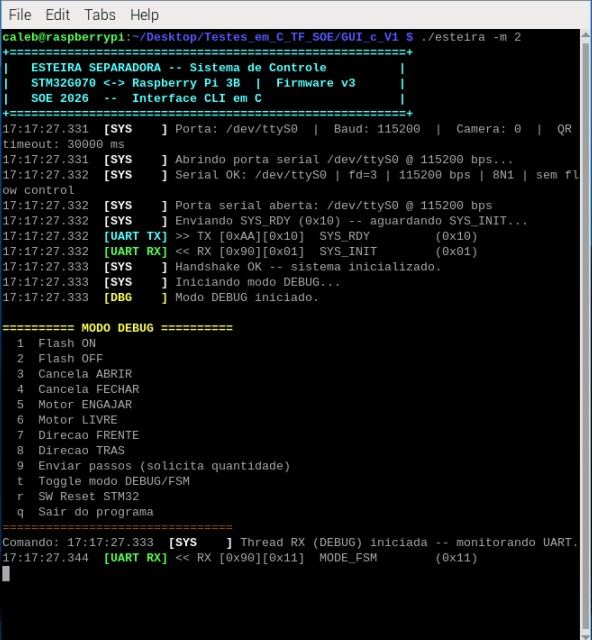
\includegraphics[width=\linewidth]{figuras/tabela_terminal.jpeg}
    \caption{Menu do modo DEBUG exibido no terminal (\texttt{debug.c}).}
    \label{fig:debug_menu}
\end{figure}

\begin{figure}[!htpb]
    \centering
    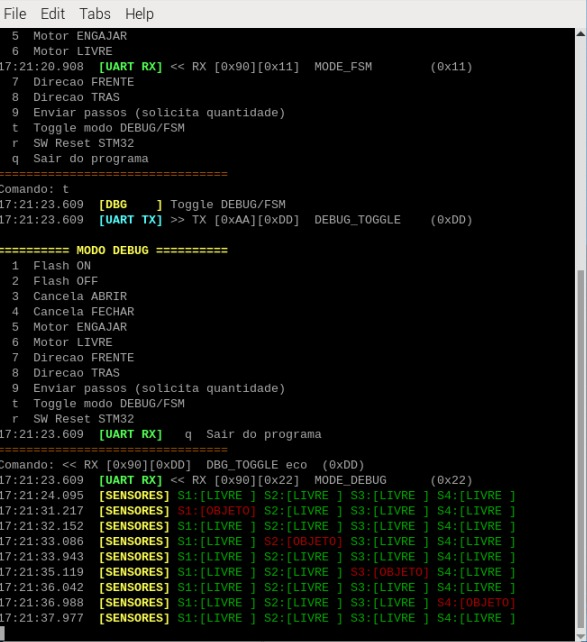
\includegraphics[width=\linewidth]{figuras/telemetria_sensores.jpeg}
    \caption{Telemetria dos sensores S1--S4 em tempo real
             (\texttt{SENS\_STATUS}, \texttt{0x55}).}
    \label{fig:sensor_telemetry}
\end{figure}

\paragraph{Módulo \texttt{camera.cpp} — captura e decodificação de QR.}
Único módulo em C++, com funções exportadas via \texttt{extern "C"} para
compatibilidade com os demais módulos C. Captura \textit{frames} em
640$\times$480\,px via \texttt{cv::VideoCapture}, converte para escala de
cinza e entrega o \textit{buffer} ao ZBar em formato \texttt{Y800}. O
\textit{parser} interno \texttt{parse\_qr\_text()} busca primeiro o campo
\texttt{Destino:} no texto do QR e, em seguida, realiza varredura linear de
tokens hexadecimais, garantindo compatibilidade com diferentes formatos.
A correspondência é \texttt{0xDA} $\to$ Rota~A e \texttt{0xDB} $\to$
Rota~B.

\paragraph{Módulo \texttt{log.c} — sistema de log.}
Todas as mensagens seguem o formato \texttt{HH:MM:SS.mmm [CATEGORIA]
mensagem}, com \textit{timestamp} gerado via
\texttt{clock\_gettime(CLOCK\_REALTIME)} e categorias codificadas por cores
ANSI (\texttt{[UART TX]}, \texttt{[UART RX]}, \texttt{[FSM]},
\texttt{[CAM]}, \texttt{[DBG]}, \texttt{[SYS]}, \texttt{[ERR]}).

\paragraph{Gerador de códigos QR.}
Para a criação dos códigos QR utilizados nos testes, foi desenvolvido um
script Python auxiliar (\texttt{gerar\_qrcodes.py}) que lê um arquivo JSON
com as informações das peças e gera as imagens correspondentes. Cada código
QR codifica o nome da peça e o destino (endereço hexadecimal utilizado pela
FSM) conforme o formato arbitrado pela dupla.

Todos os arquivos podem ser encontrados no repositório do
projeto~\cite{ref:github_soe}.